\chapter{Variational Auto-encoders and Generative Adversarial Networks}

\section{Variational Auto-Encoders}
% Authors: Yu Cao, Evgenii Nikitin
% Editor: Aishwarya Budhkar 
% Lab date: 4/16/2019
\begin{figure}[H]
    \centering
    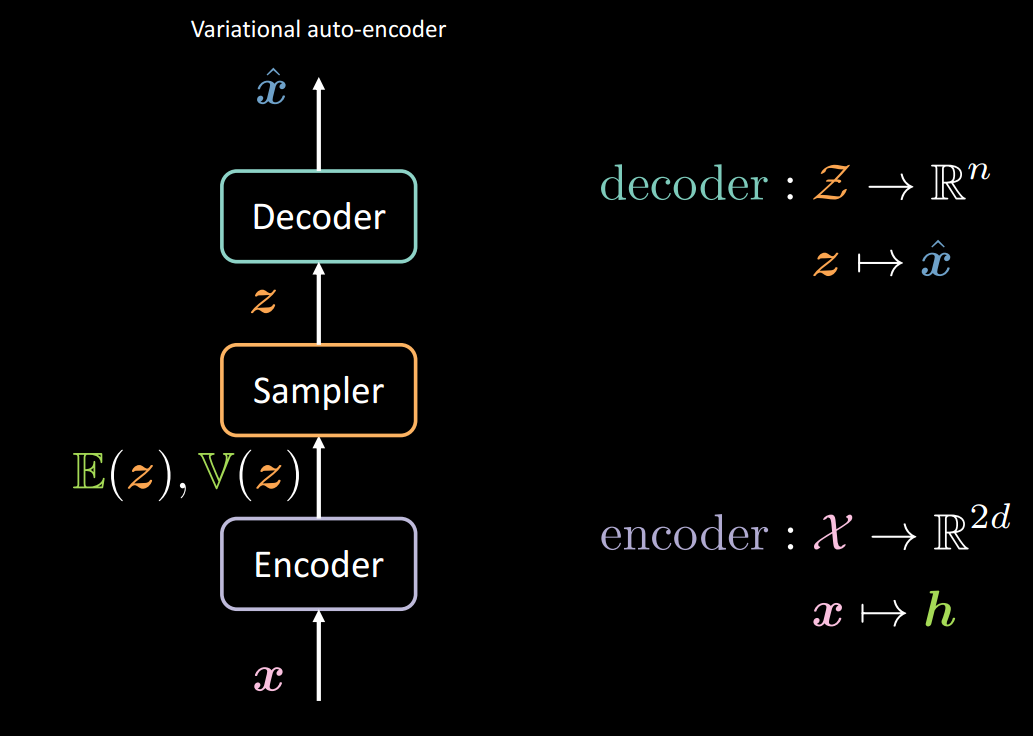
\includegraphics[width=0.7\textwidth]{labs/10/images/vae.png}
    \caption{Architecture of Variational Autoencoder}
    \label{fig:vae}
\end{figure}
 
There are two types of Auto-Encoders: Over-complete and Under-complete. A type of constraint that can be applied which is information bottleneck is reduction in the size of intermediate layer which leads to under-complete auto-encoder. In over-complete auto-encoder there is larger intermediate layer so we can extract better meaningful features. Variational autoencoders (VAE) inherit the architecture of the traditional autoencoders -- they also consist of two main components: encoder and decoder. However, there is a key difference between them -- while encoder in vanilla AE outputs a hidden representation $h$ of the input $x$, VAE encoder produces two vectors -- expectation $E(z)$ and variance $V(z)$ over latent variable $z$ (Figure \ref{fig:vae}). This property allows us to produce stochastic representations of the input. This is achieved by sampling a vector from the standard normal distribution with zero mean and unit variance and shifting and rescaling vector elements according to estimated $E(z)$ and $V(z)$ respectively:
\begin{align*}
    \vect{z'} &= \mathop{\mathbb{E}}(\vect{z}) + \vect{\epsilon} \odot \sqrt{\mathop{\mathbb{V}}(\vect{z})} \\
    \vect{\epsilon} &\sim \mathcal{N}(0, \mathcal{I}_d)
\end{align*}

After that, sampled representation $z'$ is decoded into output $\hat{x}$. In order to make sure that this output is close to the input $x$, we introduce a reconstruction component of the loss function -- $\ell(x,\hat{x})$ (e.g., MSE loss or binary cross-entropy depending on the nature of the data).

\begin{figure}[H]
    \centering
    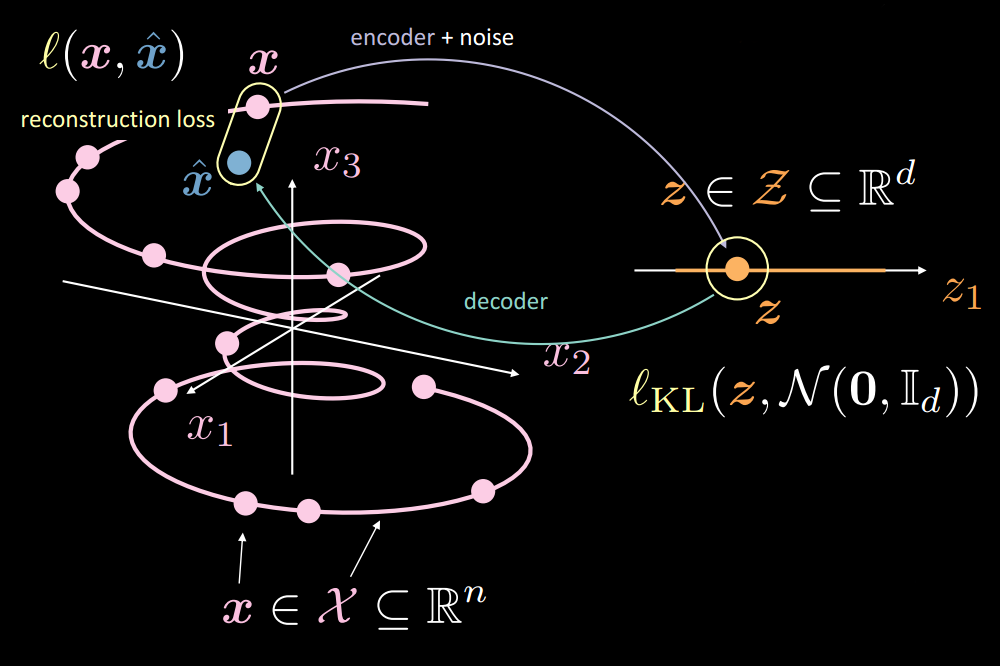
\includegraphics[width=0.7\textwidth]{labs/10/images/vae_expl.png}
    \caption{Visualization of encoding and decoding processes}
    \label{fig:vae_expl}
\end{figure}

However, as there is no limit on the values of $E(z)$ and $V(z)$, the encoder can learn to push different training samples very far apart in the latent space (Figure \ref{fig:bubbles_rec}), effectively reconstructing the training data. In order to avoid this, we introduce a constraint by adding KL-divergence component to the loss function. 
\begin{align*}
    \ell(x, \hat{x}) = \ell_{rec} + \beta \ell_{KL} (z, \mathcal{N}(0, \mathcal{I}_d)) \simeq \ell_{rec} + \beta\sum_{i=1}^d (\mathop{\mathbb{V}}(\vect{z}) - \log{\mathop{\mathbb{V}}(\vect{z})} - 1 + \mathop{\mathbb{E}}(\vect{z})^2)_i
\end{align*}

Intuitively, this new term forces learned representations of the training samples to have unit variance and to be as close to zero as possible (Figure \ref{fig:bubbles_kl}). $\beta$ is a hyperparameter that controls the tightness of the constraint. To sum up, reconstruction loss ensures that the different "bubbles" do not overlap, so we can still reconstruct the different inputs, while KL-divergence loss confines them to the most compact space possible. This feature of VAE leads to a smooth learned latent spaces, allowing interpolation between the different samples and classes.

\begin{figure}[H]
    \centering
    \begin{subfigure}[b]{.45\linewidth}
    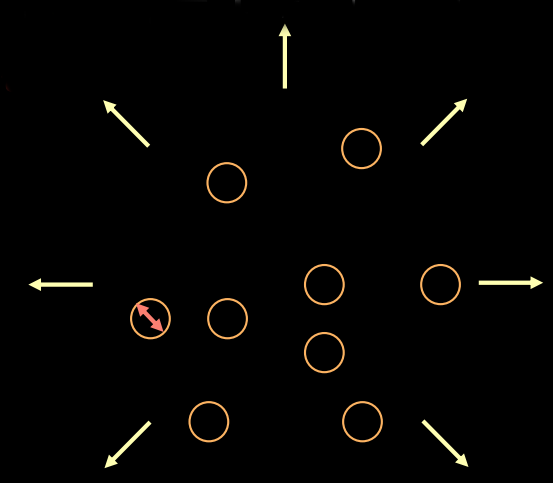
\includegraphics[width=\linewidth]{labs/10/images/bubbles_rec.png}
    \caption{Samples get pulled apart by reconstruction loss}\label{fig:bubbles_rec}
    \end{subfigure}
    \begin{subfigure}[b]{.45\linewidth}
    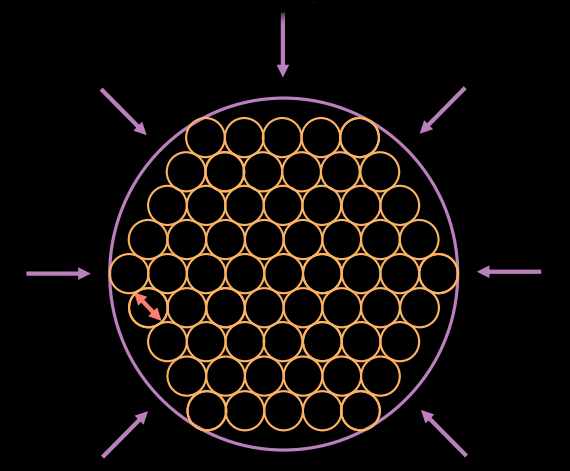
\includegraphics[width=\linewidth]{labs/10/images/bubbles_kl.png}
    \caption{Samples get pushed towards zero by KL-divergence loss}\label{fig:bubbles_kl}
    \end{subfigure}
    \caption{Effects of the different loss components}
    \label{fig:bubbles}
\end{figure}

\section{Generative Adversarial Network}
\subsection{Introduction}
\begin{figure}
    \centering
    \includegraphics[width=0.7\textwidth]{"labs/10/images/VAE and GAN".png}
    \caption{Architecture of GAN}
    \label{fig:my_label}
\end{figure}

As we can see in the figure. The GAN model is similar to the VAE model.

Consider a guy who makes fake money. The $\hat{x}$ produced by sampler+generator can be thought as the fake money he makes. Then he sends the money to someone(the discriminator) who wants to tell apart fake money from the genuine one ($x$). If the fake money is not 'good' enough, the discriminator will sends some feedback(sent through backpropagation) and the guy can improve his skills(gradient descent), until the discriminator can not tell apart the fake one from the genuine one. 

From the sampler we come up with some noise. On top of the sampler we have the generator which tries to create authentic data, similar to the decoder to VAE, both of which are generative networks. From the generator we get our estimate $\hat{x}$on the manifold. The estimate, together with our real $x$, is sent to a discriminator which tries to tell apart $x$ from $\hat{x}$ that is difference between fake and actual values. We can optimize the generator depending on what fools and does not fool the discriminator

For generator, We map the latent space to input space $\begin{array}{r}{G : \mathcal{Z} \rightarrow \mathbb{R}^{n}}, {z \mapsto \hat{x}}\end{array}$

For discriminator, we go from the original input ($x$) or the crafted input ($\hat{x}$) to a learned loss. $\begin{aligned} D : & \mathbb{R}^{n} \rightarrow(0,1) & x \vee \hat{x} \mapsto \ell \end{aligned}$

\subsection{Model illustration}

\begin{figure}
    \centering
    \includegraphics[width=0.7\textwidth]{"labs/10/images/GAN illustration".png}
    \caption{Visualization of encoding and decoding process}
    \label{fig:my_label}
\end{figure}

We start from a random variable in the hidden space. Then we get our $\hat{x}$ from the generator. Note that in the GAN setting, we do not know our data manifold, so there will be no way trying to proximate $\hat{x}$ to data manifold. We apply our discriminator on both the crafted data and real data. We train our discriminator so that it can tell apart the two. On the other hand, we get the gradient, so that we can make the generated data as close to the real data manifold as possible. \\ 


When training GAN, we don't use a so called loss function because we not not trying to minimizing it. Instead, we use the following value function.

$$V(D, G)=\mathbb{E}_{\boldsymbol{x} \sim p_{\text { data }}(\boldsymbol{x})}[\log D(\boldsymbol{x})]+\mathbb{E}_{\boldsymbol{z} \sim p_{\boldsymbol{z}}(\boldsymbol{z})}[\log (1-D[G(\boldsymbol{z})])]$$
$$\min _{G} \max _{D} V(D, G)$$

The above function reaches an equilibrium (Nash equilibrium ) between the performance of the discriminator and the performance of the generator. When the two modules reach their best performance together, the discriminator should be able to tell apart fake data and real data, and the generator will be generating perfect data.